\section{Detection Algorithm}

Our goal is to detect the home network bottleneck in a scalable, easily installable manner, without introducing excessive probing traffic. Furthermore, we can take advantage of collaborative devices in the home, such as smart phones, other laptops, and collaborative gateways (if available). To this end, we present a bandwidth bottleneck detection algorithm. Currently implemented as a python tool, in the future, we will port this algorithm to a browser extension to perform low traffic bandwidth and latency tests.

\subsection{Bandwidth Bottleneck}
\label{bandwidth}

We compare the available TCP bandwidth of individual segments (home, access, end to end) to pinpoint the tight link. Consider that we have an external server to test to, and a wireless test client inside the home. Now, we can perform measurements if either of the two devices are also present: (a) collaborative gateway; (b) user controlled collaborative test device

\textbf{Collaborative Gateway:} which can form an end point for bandwidth measurements
\begin{itemize}%[noitemsep,topsep=0pt,parsep=0pt,partopsep=0pt]
\item Measure wireless TCP bandwidth between client and router.
\item Start measuring access TCP bandwidth between router and client.
\item Stop measurement as soon as the access throughput exceeds wireless throughput. If this happens, wireless is bottleneck. Else, access is bottleneck.
\end{itemize}
This algorithm was evaluated in both the testbed and real networks with OpenWRT gateways (Section \ref{evaluation})

\textbf{Collaborative Test Device:} The main idea here is to direct the user to place a control device, such as a smartphone, in the home at a good position ensuring a good wireless throughput, to conduct tests using that device as a reference. %See figure \ref{fig:two-device}
\begin{itemize}%[noitemsep,topsep=0pt,parsep=0pt,partopsep=0pt]
\item Place control end host device (B) near home gateway and ensure it has a better throughput than test device (A) to the server (S). Throughput of test device = AS; throughput of control device = BS.
\item Measure bidirectional wireless bandwidth between test and control devices, i.e. throughput AB (or BA).
\item If AS < AB, then access link is bottleneck.%If wireless bandwidth between the two devices (AB) exceeds end to end throughput of test device (AS), then access link is the bottleneck. i.e., 
\item If AS < AB < BS, then wireless link is bottleneck.%%If wireless bandwidth between the two devices (AB) is less than the end to end throughput of control device (BS), but more than the end to end throughput of the test device (AS), then wireless link of test device is the bottleneck. i.e.,
\end{itemize}

%\begin{figure}[!ht]
%\begin{center}
%    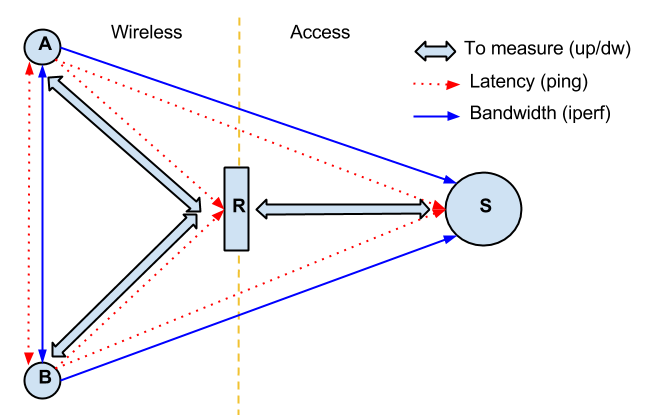
\includegraphics[width=3.2in,height=1.9in]{two-device.png}
%\end{center}
%\caption{Bandwidth and Latency measurements using two collaborating devices.}
%\label{fig:two-device}
%\end{figure}

\subsection{Latency Bottleneck}
\label{latency}

This algorithm is based on the observation that the buffers of a tight link are full during an end to end flow. One way to check for this is to compare the increase in RTT over the home and access segment when a link is being probed. Another approach to detect tight links is by differentially overflowing the wireless and the access link and comparing the delay observed at the listener. This can be done using STAB \cite{stab}, a successor of the pathChirp \cite{pathchirp}.

We use one end host device to send a train of pairs of large packets followed immediately by a small packet . The large packet has a limited TTL and is dropped at a particular hop based on that TTL. So it only saturates the link before it was dropped. The listener (end host server) records the timing of the small packet to diagnose the thin bottleneck link at which the big packet with limited TTL got dropped. If the access link is the uplink bottleneck, we will see that TTL=1 packets which only saturate the wireless result in smaller timings at the listener than the packet trains with large TTL which also covers the access network.